\documentclass{article}
\usepackage[margin=2.5cm]{geometry}
\usepackage{amsmath}
\usepackage{subcaption}
\usepackage{graphicx}
\usepackage{hyperref}
\hypersetup{colorlinks=true,linkcolor=black,citecolor=black,urlcolor=black}
\urlstyle{same}

\title{Computing normalization factors for single-cell RNA-seq data: avoiding problems with zero counts}
\author{Aaron Lun and Karsten Bach}

\begin{document}
\maketitle

\section{Introduction}
Single-cell RNA sequencing (scRNA-seq) is a powerful technique that allows researchers to characterize the gene expression profile of single cells.
From each cell, mRNA is isolated, reverse-transcribed and subjected to massively parallel sequencing \cite{stegle2015computational}.
The sequencing reads are then mapped to a reference genome, whereby the number of reads mapped to each gene can be used to quantify the expression of that gene.
Alternatively, transcript molecules can be counted directly using unique molecular identifiers (UMIs) \cite{islam2014quantitative}.
Count data can be analyzed to identify new cell subtypes and to detect highly variable or differentially expressed (DE) genes between cell subpopulations.
This type of single-cell resolution is not possible with bulk RNA sequencing of cellular populations.
However, the downside is that the counts often contain high levels of technical noise with many ``drop-outs'', i.e., zero or near-zero values.
This is due to the difficulties in sequencing low amounts of RNA per cell, which decreases the capture efficiency during library preparation.
Moreover, the capture efficiency often varies from cell to cell, such that counts cannot be directly compared between cells.

Normalization of the scRNA-seq counts is a critical step that corrects for differences in capture efficiency between cells.
Two broad classes of normalization approaches are available -- those using spike-in RNA sets, and those using the counts for cellular RNA.
In the former, the same quantity of spike-in RNA is added to each cell prior to library preparation \cite{stegle2015computational}.
Any difference in the coverage of the spike-in transcripts must be caused by differences in capture efficiency between cells.
Normalization is then performed by scaling the counts to equalize spike-in coverage between cells.
For the methods using the cellular counts, the common assumption is that most genes are not DE across the sampled cells.
Counts are then scaled so that there is, on average, no fold-difference in expression between cells for the majority of genes.
This is the underlying concept of commonly used methods such as size factor \cite{anders2010differential} and trimmed mean of M-values (TMM) normalization \cite{robinson2010scaling}.
An even simpler approach involves scaling the counts to remove differences in library sizes between cells.

The type of normalization that can be used often depends on the characteristics of the data set.
In some data sets, spike-in data may not be present -- for example, droplet-based protocols \cite{klein2015droplet,macosko2015highly} do not allow spike-ins to be easily incorporated.
This obviously precludes the use of spike-in normalization.
The methods based on cellular counts can be applied more generally but have their own deficiencies.
Normalization by library size is insufficient when DE genes are present, as composition biases can introduce spurious differences between cells \cite{robinson2010scaling}.
Size factor or TMM normalization are more robust to DE but rely on the calculation of ratios of counts between cells.
This is not straightforward in scRNA-seq data, where the high frequency of drop-out events interferes with stable normalization.
A large number of zeroes will result in nonsensical size factors or undefined M-values in the TMM method.
One could proceed by removing the offending genes during normalization for each cell, but this may introduce biases if the number of zeroes varies across cells.

Correct normalization of scRNA-seq data is essential as it determines the validity of all downstream quantitative analyses.
In this article, we describe a deconvolution approach that improves the accuracy of the non-DE (i.e., size factor or TMM) normalization methods.
Briefly, normalization is performed on pooled counts for multiple cells, where the incidence of problematic zeroes is reduced
    -- the pooled size/normalization factors are then deconvolved back to those for the individual cells.
Using a variety of simple simulations, we demonstrate that our approach outperforms the direct application of those normalization methods for count data with many zeroes.
We also show a similar difference in behaviour on several real data sets, where deconvolved normalization yields results that are more biologically relevant.
These results suggest that our approach is a viable alternative to existing methods for general normalization of scRNA-seq data.

\section{Existing normalization methods fail with zero counts}

\subsection{The origin of zero counts in scRNA-seq data}
The high frequency of zeroes in scRNA-seq data is driven by both biological and technical aspects.
Gene expression is highly variable across cells due to cell-to-cell heterogeneity and phenomena like transcriptional bursting \cite{marinov2014singlecell}.
Such variability is likely to result in zero counts for the lowly expressed genes.
It is also technically difficult to process low quantities of input RNA into sequenceable libraries.
This results in high dropout rates whereby low-abundance transcripts are not captured during library preparation \cite{brennecke2013accounting}.

At this point, it is important to distinguish between stochastic and systematic zeroes.
Systematic zeroes refer to genes that are constitutively silent in a cell (sub)population, such that the count must be zero for all cells in that population.
These are generally not problematic as they contain no information and can be removed prior to normalization.
Stochastic zeroes are found in genes that are actively expressed but obtain counts of zero in some cells due to sampling stochasticity.
These genes may contain information about the relative differences between cells, so removing them prior to normalization may introduce biases.

\subsection{A brief description of existing non-spike-in methods}
Here, we only consider those normalization methods not based on spike-in data.
This is motivated by the desire to obtain a general method that can be applied in all data sets.
In particular, we will review three approaches that are commonly used for RNA-seq data -- size factor, TMM and library size normalization.

Size factor normalization was originally introduced as part of the DESeq package for differential expression \cite{anders2010differential}.
It first constructs an ``average'' reference library, in which the ``count'' for each gene is defined as the geometric mean of the counts for that gene across all real libraries.
Each real library is then normalized against this average.
Specifically, for each gene, it computes the ratio of the count in each library to that in the average library.
The size factor for each library is defined as the median of this ratio across all genes.
This value represents the extent to which the counts in that library should be downscaled, 
    in order to eliminate any systematic differences in expression between libraries for the majority of (assumed) non-DE genes.

TMM normalization was introduced as part of the edgeR package for differential expression \cite{robinson2010edgeR}.
It selects one library to be a reference, and normalizes each other library against the reference.
Specifically, for each library, M-values (i.e., library size-adjusted log$_2$-ratios in expression) are computed against the reference for all genes.
The genes with the most extreme M-values are trimmed away.
High- or low-abundance genes are similarly removed.
The weighted mean of the remaining M-values is computed, where the weighting is performed according to the asymptotic variance of each M-value.
This is used to define the normalization factor for each library as $2^x$, where $x$ is the weighted mean for that library.
The normalization factor represents the downscaling required to eliminate systematic differences between libraries, additional to that required to equalize the library sizes.
Taking the product of the normalization factor and library size for each library (i.e., the effective library size) yields a value that is functionally equivalent to the size factor.

Both size factor and TMM normalization assume that most genes are not DE between libraries.
Any systematic difference in expression across the majority of genes is treated as bias.
This is duly incorporated into the size/normalization factors and removed upon scaling.
If the non-DE assumption does not hold, the computed factors will not be accurate.
In addition, both methods perform poorly in the presence of a large number of zeroes.
For size factor normalization, the geometric mean is equal to zero for genes with a zero count in any library, such that the ratios for that gene become undefined.
Conversely, a library with zero counts for many genes may have a size factor of zero, which precludes any sensible scaling.
For TMM normalization, M-values are undefined when the count in either library is zero.
In such conditions, both methods typically require \textit{ad hoc} workarounds such as the removal of zero counts within each library.

Finally, library size normalization is another commonly used approach for RNA-seq data.
This involves scaling the counts such that the library size is the same across libraries.
While simple, this approach is not robust in the presence of DE genes \cite{robinson2010scaling}.
One can imagine a scenario where a single gene is strongly upregulated in one library compared to another.
This increases the size of the first library, as more reads are generated from the upregulated gene.
Normalization by library size will then scale up the counts for the second library to compensate.
This introduces spurious differences in the counts between libraries for the non-DE genes.
The likely presence of DE in real data means that library size normalization is often inappropriate.

\subsection{Performance of existing methods on simulated data with zeroes}
To test the performance of existing methods, simulated scRNA-seq data was generated with DE genes and a large number of stochastic zeros.
Consider a cell $j$ in a subpopulation $s$.
This subpopulation may represent cell type or some other biological condition, e.g., drug treatment. 
For each gene $i$ in this cell, the count $y_{ij}$ was sampled from a negative binomial (NB) distribution with mean $\theta_{j}\lambda_{is}$.
The $\theta_{j}$ term represents cell-specific biases (e.g., in capture efficiency) that must be normalized out, 
    and is sampled for each cell such that 
\[
\log_2(\theta_j) \sim \mathcal{N}(0, 0.25) \;.
\]
The $\lambda_{is}$ term denotes the expected number of transcripts of gene $i$ for cells in subpopulation $s$.
It is defined as $\lambda_{is}=\phi_{is}\lambda_{i0}$ where $\phi_{is}$ represents the DE for this gene in this subpopulation, and 
\[
\log_2(\lambda_{i0}) \sim \mbox{Uniform}(3, 6) \;.
\]
This recapitulates the spread of abundances in real data.
The NB dispersion is defined for each gene as 
\[
    \varphi_i = 2 + \frac{100}{\lambda_{i0}}
\]
to represent a decreasing mean-dispersion trend.
Large values for $\varphi_i$ are consistent with the high levels of technical noise and biological heterogeneity in scRNA-seq studies,
    and ensure that a large number of stochastic zeroes are generated.
Approximately 30-50\% of all counts are zero in each simulated library.

The simulation design involves 10000 genes for three subpopulations of 250 cells each.
For each subpopulation, a unique set of $G$ genes was randomly chosen.
DE was introduced by setting $\phi_{is}$ to some constant $\phi_s$ for $p_s$ of the $G$ genes (i.e., upregulated) and to $\phi_s^{-1}$ for the rest (downregulated).
The value of $\phi_s$ was set to 5 for all $s$, while $p_s$ was set to 20, 50 and 80\% for the first, second and third subpopulations, respectively.
This provides each subpopulation with a unique expression signature containing different numbers of DE genes in each direction.
Simulations were performed for $G = 0$ (no DE), 1000 (moderate DE) and 3000 (strong DE).
The simulation was also repeated with $G$ set to 3000, $p_s$ set to 50\% for all $s$ and $\phi_{s}$ set to 2, 5 and 10 for the first, second and third subpopulations, respectively.
This represents an alternative scenario where the number of DE genes in either direction is the same but the magnitude of DE is different between subpopulations.
For all scenarios, simulated data was generated by sampling NB-distributed counts as described.

Size factor, TMM and library size normalization were applied to this data.
For size factor normalization, the geometric mean was computed by replacing all zero counts with unity.
Zero counts were also removed within each library prior to calculation of the size factor.
For TMM normalization, all undefined M-values were removed prior to trimming and calculation of the normalization factor for each library.
The corresponding size factor was defined as the effective library size, i.e., the product of the library size and the normalization factor for each library.
The true size factor for each cell is $\theta_j$, as it represents the extent of scaling required to remove cell-specific biases.
For library size normalization, the total library size was used directly as the size factor for each cell.
Estimated size factors were then compared to the true values for all cells.

All methods yield size factors that systematically deviate from the true values (Figure~\ref{fig:existing_sim}).
For size factor and TMM normalization, large size factors are consistently underestimated while small size factors are overestimated.
This is a consequence of removing stochastic zeroes prior to normalization.
Cells with low $\theta_j$ are likely to contain more stochastic zeroes, as the mean of the sampling distribution for the counts is lower.
If these zeroes are removed prior to size factor normalization, the median ratio will be computed from the remaining non-zero counts.
This shifts the median upwards and results in overestimation.
Similarly, the distribution of M-values will be shifted towards positive values upon removal of zeroes.
This is because stochastic zeroes represent sampled values below some non-zero mean, and would generally correspond to negative M-values.
Their removal increases the (trimmed) mean of M-values and biases the estimate of the TMM normalization factor.
The converse applies to cells with large $\theta_j$.
Size factors have a relative interpretation, so overestimation of small $\theta_j$ will lead to a concomitant underestimation for large $\theta_j$.

\begin{figure}[tbp]
\begin{minipage}{0.33\textwidth}
\includegraphics[width=\textwidth,trim=0mm 12mm 2mm  5mm,clip]{results/size_1.pdf}
\includegraphics[width=\textwidth,trim=0mm 12mm 2mm 15mm,clip]{results/size_2.pdf}
\includegraphics[width=\textwidth,trim=0mm 12mm 2mm 15mm,clip]{results/size_3.pdf}
\includegraphics[width=\textwidth,trim=0mm  5mm 2mm 15mm,clip]{results/size_4.pdf}
\subcaption{}\label{subfig:size_sim}
\end{minipage}
\begin{minipage}{0.33\textwidth}
\includegraphics[width=\textwidth,trim=0mm 12mm 2mm  5mm,clip]{results/TMM_1.pdf}
\includegraphics[width=\textwidth,trim=0mm 12mm 2mm 15mm,clip]{results/TMM_2.pdf}
\includegraphics[width=\textwidth,trim=0mm 12mm 2mm 15mm,clip]{results/TMM_3.pdf}
\includegraphics[width=\textwidth,trim=0mm  5mm 2mm 15mm,clip]{results/TMM_4.pdf}
\subcaption{}\label{subfig:tmm_sim}
\end{minipage}
\begin{minipage}{0.33\textwidth}
\includegraphics[width=\textwidth,trim=0mm 12mm 2mm  5mm,clip]{results/lib_1.pdf}
\includegraphics[width=\textwidth,trim=0mm 12mm 2mm 15mm,clip]{results/lib_2.pdf}
\includegraphics[width=\textwidth,trim=0mm 12mm 2mm 15mm,clip]{results/lib_3.pdf}
\includegraphics[width=\textwidth,trim=0mm  5mm 2mm 15mm,clip]{results/lib_4.pdf}
\subcaption{}\label{subfig:lib_sim}
\end{minipage}
\caption{
    Performance of existing normalization methods on the simulated data with DE genes and stochastic zeroes.
    The size factor estimate for each cell is plotted against its true values for (\subref{subfig:size_sim}) size factor,
        (\subref{subfig:tmm_sim}) TMM and (\subref{subfig:lib_sim}) library size normalization.
    Simulations were performed with no DE (first row), moderate DE (second row), strong DE (third row) and varying magnitudes of DE (fourth row).
    Axes are shown on a log-scale for visibility.
    The red line represents equality between the estimated and true factors.
    Cells in the first, second and third subpopulations are shown in black, blue and orange, respectively.
}
\label{fig:existing_sim}
\end{figure}

The presence of DE genes results in a further deterioration in performance of all methods (Figure~\ref{fig:existing_sim}).
The divergence between the true and estimated size factors increases as the number of DE genes increases,
    consistent with a decrease in the validity of the non-DE assumption required by all methods.
To illustrate, consider the strong DE simulation.
Across the three subpopulations, there are 9000 genes involved in subpopulation-specific signatures, i.e., 90\% of all genes exhibit DE within this data set.
An assumption of a non-DE majority of genes is clearly invalid in this scenario.
Any systematic differences in expression between cells of different subpopulations will now include genuine DE in addition to cell-specific biases.
Subsequently, the magnitude of DE will be incorporated in the size factors computed from each method, such that they are no longer accurate estimates of $\theta_j$.
The estimates also split into three distinct groups in Figure~\ref{fig:existing_sim}, each corresponding to a different subpopulation.
Size factors tend to be overestimated for subpopulations with more DE, as the increased expression of upregulated genes drags up the median ratio/trimmed mean.

\section{Improving normalization accuracy with deconvolution}

\subsection{Overview of the deconvolution strategy}
The aim of the deconvolution strategy is to normalize on summed expression values from pools of cells.
Summation across cells results in fewer zeroes, which means that the ensuing normalization is less susceptible to the errors observed for existing methods.
While normalization accuracy is improved, the estimated size factors are only relevant to the pools of cells.
This is not particularly interesting for downstream analyses focusing on single cells.
In order to be useful, the size factor for each pool is deconvolved back into the size factors for its constituent cells.
This ensures that cell-specific biases can be properly normalized.

\subsection{Summation and deconvolution with linear equations}
Define the size-adjusted expression of gene $i$ as $\pi_{ij} = y_{ij}T_j^{-1}$, where $T_j$ is the total library size for cell $j$.
The expectation of $\pi_{ij}$ can then be written as $\theta_j\lambda_{is} T_j^{-1}$.
Further assume that we have an arbitrary set of cells $\mathcal{S}_k$.
Denote the sum of $\pi_{ij}$ across $\mathcal{S}_k$ as $s_{ik}$ for gene $i$.
The values of $s_{ik}$ across all genes constitute an overall expression profile for the pool of cells corresponding to $\mathcal{S}_k$.
The expectation of $s_{ik}$ is equal to 
\[
    E(s_{ik}) = \lambda_{is} \sum_{j \in \mathcal{S}_k} \theta_j T_j^{-1}\;.
\]
Define $u_{i}$ as the mean of expression values for gene $i$ across all $N$ cells in the entire data set.
The values of $u_{i}$ across all genes represent the expression profile for an averaged reference pseudo-cell.
The cell pool for set $\mathcal{S}_k$ is then normalized against this reference pseudo-cell.
Let $r_{ik}$ denote the ratio of $s_{ik}$ to $u_{i}$ for a non-DE gene $i$.
The expectation of $r_{ik}$ represents the size factor for the pooled cells in $\mathcal{S}_k$, and is written as
\begin{equation}
    E(r_{ik}) \approx \frac{E(s_{ik})}{E(u_{i})} 
    = \frac{\sum_{\mathcal{S}_k} \theta_j T_j^{-1}}{ N^{-1} \sum_{\mathcal{S}_0} \theta_j T_j^{-1}} 
    = \frac{\sum_{\mathcal{S}_k} \theta_j T_j^{-1}}{C}
    \label{eqn:linear_single}
\end{equation}
where $C$ is a constant that does not depend on the gene, cell or set $\mathcal{S}_k$.
The above approximation is valid if the variance of the sums is low -- 
    this should be the case for large sets, as the variability relative to the mean should decrease due to the law of large numbers.
$E(r_{ik})$ is estimated by taking any robust average (in this case, the median) of $r_{ik}$ across $i$.
Robustness protects the average against DE genes with extreme ratios.

The estimated value of $E(r_{ik})$ for the set can be used to obtain estimates for $\theta_j$ for each cell.
A linear equation is set up based on the expression in Equation~\ref{eqn:linear_single}, 
by replacing $E(r_{ik})$ with its estimate and treating the $\theta_j T_j^{-1}$ as unknown parameters to be estimated.
The constant $C$ can be set to unity and ignored, as it does not contribute to the relative differences between size factors.
Repeating the estimation of $E(r_{ik})$ for different sets of cells in $\mathcal{S}_{ik}$ will generate an overdetermined system of linear equations, 
    in which the $\theta_j T_j^{-1}$ for each $j$ is represented at least once.
This system can then be solved with least-squares methods to obtain estimates of $\theta_j T_j^{-1}$ for all cells.
Multiplication by $T_j$ for each cell will then yield an estimate of $\theta_j$.

This approach may seem somewhat circuitous, given that $\theta_j$ could be estimated directly from the counts for each individual cell.
However, summation reduces the number of stochastic zeroes that cause problems in existing methods.
As a result, ratios computed from pooled expression profiles are more accurate.
This improvement will propagate back to the $\theta_j$ estimates for each $j$ when the linear system is solved.

\subsection{Obtaining sensible least-squares solutions}
The linear system can be solved using standard methods, such as those based on the QR decomposition.
However, with such methods, it is theoretically possible to obtain negative estimates for $\theta_j$.
Such values are obviously nonsensical as counts cannot be scaled to negative values.
One situation in which this might occur involves data with a large spread of $\theta_jT_j^{-1}$ values, 
    such that the true value of $\theta_jT_j^{-1}$ is already close to zero for some cells.
Errors in estimation may then be sufficient to push the estimated $\theta_j$ below zero.
Protection is provided by using linear inverse models \cite{soetaert2009limsolve} to constrain the estimates to non-negative values.
This will not provide sensible estimates for the offending cells -- these are set to zero and should be removed --
    but will ensure that the estimates for other cells are not distorted by negative values elsewhere in the system.

Note that counts could be summed rather than size-adjusted expression values.
This means that the solution of the linear system will directly yield estimates of $\theta_j$.
However, we use size-adjusted values to ensure that the sum is not dominated by a small number of very large libraries.
Information from each cell will then be weighted equally when computing the median ratio for each set, regardless of library size.
It also reduces the risk of obtaining negative estimates for very small libraries.
Such libraries have very small $\theta_j$ and would be unduly influenced by (relatively) large estimation errors for cells with larger libraries.

\subsection{Clustering to weaken the non-DE assumption}
This approach makes some moderately strong assumptions regarding the nature of DE across the data set.
The use of the median is only valid when less than 50\% of genes are DE in any direction in the cell pool compared to the reference pseudo-cell,
    i.e., less than 50\% of genes can be upregulated and less than 50\% of genes can be downregulated.
If more DE genes are present, the median will not represent a robust average across non-DE genes.
This condition generally requires a proportion of genes to be constantly expressed across all cells in the data set 
    -- otherwise, all genes would be DE against the average in at least one pseudo-cell -- 
    and is only guaranteed to be true when that proportion is equal to or greater than 50\% of all genes.
This is similar to that required for size factor normalization where an average reference is also used.

To reduce the strength of the non-DE assumption, cells can be clustered based on their expression profiles.
The deconvolution method is then applied to the cells in each cluster $\mathcal{C}$ separately,
    where the sets $\mathcal{S}_k$ are nested within each $\mathcal{C}$.
This normalizes each cell pool of $\mathcal{S}_k$ to a cluster-specific reference pseudo-cell for $\mathcal{C}$,
    yielding a cluster-specific size factor of $f_{j}'$ for cell $j \in \mathcal{C}$ after deconvolution.
These cluster-specific size factors must be rescaled before they can be compared between clusters.
To do so, the reference pseudo-cells for all clusters are normalized against each other.
This is done by selecting a single ``baseline'' pseudo-cell against which all other pseudo-cells are normalized.
The median ratio $\tau_{\mathcal{C}}$ of the expression values is computed for the pseudo-cell of each cluster against the baseline pseudo-cell
    (obviously, the cluster chosen as the baseline will have $\tau_{\mathcal{C}}=1$).
The overall size factor for cell $j$ in cluster $c$ is subsequently defined as $f_j = f_{j}'\tau_{\mathcal{C}}$.

The use of within-cluster normalization reduces the number of DE genes, as all cells in each cluster have similar expression profiles.
This avoids inaccurate estimation of the size factors due to violations of the non-DE assumption.
Moreover, the pseudo-cells are normalized in pairwise comparisons to a baseline.
This weakens the assumption as a non-DE majority is only required across pairs of pseudo-cells/clusters, rather than across the entire data set.
For example, in the simulation with varying magnitude of DE, only 60\% of genes are DE between any two subpopulations, while 90\% of genes exhibit DE across all subpopulations.

Any clustering technique can be used to group cells with similar expression profiles.
We favour a correlation-based approach using $1-\rho_{xy}$ as the distance, where $\rho_{xy}$ denotes Spearman's rank correlation coefficient between the counts of cells $x$ and $y$.
Hierarchical clustering is then performed on this matrix using Ward's clustering criterion.
A dynamic tree cut is used to define clusters of cells using the dynamicTreeCut package v1.62 (\url{https://cran.r-project.org/web/packages/dynamicTreeCut/index.html}).
This is done so that each cluster contains a minimum number of cells required for stable deconvolution.
Correlation-based methods are attractive as they are insensitive to global scaling of the expression values in each cell.
Prior normalization is not required, which avoids a circular dependence between normalization and clustering.

By default, the baseline pseudo-cell is chosen from the cluster where the mean library size per cell is equal to the median of the mean per cell for all clusters
    (or, for an even number of clusters, the cluster with the smallest mean library size above the median).
This uses the mean library size as a rough proxy for cell similarity.
The baseline cluster is likely to be least dissimilar to every other cluster, which reduces the amount of DE genes during pairwise normalization.
More intelligent choices of the baseline can be used if the similarities between clusters are known, e.g., from visualization after dimensionality reduction.

\subsection{Selecting cell pools to sum}
The pool of cells in each set $\mathcal{S}_{ik}$ consists of cells with similar library sizes.
Cells in a given cluster are ordered by their total counts and partitioned into two groups, depending on whether the ranking of each cell is odd or even.
These cells are arranged in a ring, with odd cells on the left and even cells on the right.
Conceptually, one can start at the 12 o'clock position on the ring, for the largest libraries; moving clockwise through the even cells with decreasing library size;
reaching the smallest libraries at 6 o'clock; and then, continuing to move clockwise through the odd cells with increasing library size (Figure~\ref{fig:library_ring}).
For summation, a sliding window is moved cell-by-cell across this ring where each window contains the same number of cells.
These cells are used to define a single instance of $\mathcal{S}_{k}$.
Thus, each window defines a separate equation in the linear system.
The use of a ring means that the window is still defined at the smallest and largest libraries.
In contrast, sliding a window across a linear ordering of cells will result in truncated windows at the boundaries.

\begin{figure}[bt]
    \begin{center}
        \includegraphics[width=0.5\textwidth]{pics/library_ring.pdf}
    \end{center}
    \caption{
        Ring arrangement of cells ordered by library size.
        Each circle represents a cell where the size of the circle corresponds to the library size of that cell.
        Even- and odd-ranking cells lie on opposite sides, with the largest and smallest libraries at the top and bottom, respectively.
        Cells lying in a window of length 4 are highlighted in red.
        Different instances of the window are obtained by sliding the window across the ring.
    }
    \label{fig:library_ring}
\end{figure}

The pooling of cells with similar library sizes is designed to provide some robustness to DE.
Specifically, the library size is used as a rough proxy for cell similarity.
This is motivated by the fact that different cell types tend to have systematic differences in the library sizes, 
    e.g., due to type-specific differences in total RNA or capture efficiency.
Summation of cells with similar library sizes (and by implication, similar expression profiles) reduces the number of DE genes in the cell pool relative to the pseudo-cell.
This further weakens the non-DE assumption that is required by the deconvolution approach.
Note that this pooling strategy is performed on cells within a single cluster at a time.
It complements the use of clustering by protecting against any residual DE within each cluster.
This is especially true for heterogeneous populations that are difficult to partition, or in cases where larger clusters must be formed due to low numbers of cells.

% Actually doesn't matter whether or not the cells have similar expression profiles;
% DE anywhere in the data set will contaminate the average reference and break it.
% Of course, if you have 

The total number of equations in the linear system is equal to the number of cells.
The $\theta_jT_j^{-1}$ term for each cell is represented in $w$ equations, where $w$ denotes the size of the window.
By using different values of $w$, additional equations can be added to improve the precision of the estimates. 
Specifically, values of $w$ are set to 20, 40, 60, 80 and 100.
These are large enough to obtain stable sums yet small enough to maintain resolution, i.e., by ensuring that cells with very different library sizes are not summed together.
This increases the total number of equations in the system and means that each $\theta_j$ is represented in 300 equations. 

An additional set of equations is added to ensure that the system is solvable.
In each equation, the $\theta_jT_j^{-1}$ for each cell is equated to the size factor estimated directly from its single-cell counts.
These equations are assigned very low weights compared to the other equations involving summed cells, with weights of $10^{-6}$ and unity respectively.
A weighted least-squares approach is then applied to solve the linear system.
In the matrix containing the coefficients of the linear system, the incorporation of the additional equations ensures that the columns are linearly independent.
This ensures that a single solution can be obtained.
Due to their low weights, the additional equations will not contribute substantially to the weighted least-squares solution.
This means that the estimated values are driven primarily by the equations for the summed cells.

\subsection{Performance of the deconvolution approach on simulated data}
The deconvolution method provides accurate estimates of the size factor estimates in most simulation scenarios (Figure~\ref{fig:sim_cluster_DE}).
This is consistent with the reduced number of zero counts in the summed counts for each set of cells.
The median ratio for each set is more accurately computed, which improves the accuracy of the size factor estimates for the individual cells upon deconvolution.
Systematic under- or overestimation of the size factors for cells with large or small $\theta_j$ is avoided.
Some inaccuracy is observed in Figure~\ref{subfig:sumclust_3}, where the non-DE assumption is partially violated by large numbers of DE genes between subpopulations.
However, the deconvolution method is still more accurate than the existing methods in the third row of Figure~\ref{fig:existing_sim}
    -- unlike size factor or TMM normalization, the estimates here are proportional to the true values within each subpopulation, 
       and the deviation from the diagonal is smaller than that for library size normalization.

\begin{figure}[btp]
\begin{minipage}{0.48\textwidth}
    \includegraphics[width=\textwidth,trim=0mm 5mm 0mm 15mm,clip]{results/sumClust_1.pdf}
    \subcaption{}\label{subfig:sumclust_1}
\end{minipage}
\begin{minipage}{0.48\textwidth}
    \includegraphics[width=\textwidth,trim=0mm 5mm 0mm 15mm,clip]{results/sumClust_2.pdf}
    \subcaption{}\label{subfig:sumclust_2}
\end{minipage}  \\ 
\begin{minipage}{0.48\textwidth}
    \includegraphics[width=\textwidth,trim=0mm 5mm 0mm 15mm,clip]{results/sumClust_3.pdf}
    \subcaption{}\label{subfig:sumclust_3}
\end{minipage}
\begin{minipage}{0.48\textwidth}
    \includegraphics[width=\textwidth,trim=0mm 5mm 0mm 15mm,clip]{results/sumClust_4.pdf}
    \subcaption{}\label{subfig:sumclust_4}
\end{minipage}
    \caption{
        Size factor estimates from the deconvolution method in the simulation with DE genes and stochastic zeroes.
        Results are shown for scenarios with (\subref{subfig:sumclust_1}) no DE, (\subref{subfig:sumclust_2}) moderate DE, 
                (\subref{subfig:sumclust_3}) strong DE and (\subref{subfig:sumclust_4}) varying magnitude of DE.
        Cells in the first, second and third subpopulations are shown in black, blue and orange, respectively.
        Axes are shown on a log-scale, and the red line represents equality with the true factors.
    }
    \label{fig:sim_cluster_DE}
\end{figure}

One potential criticism of this approach is that it relies on clustering information.
Cluster-specific normalization might introduce artificial differences between cells in different clusters, 
    such that the statistical rigour of downstream analyses (e.g., to detect DE between clusters) would be compromised.
Such problems are avoided by normalization between the cluster-specific reference pseudo-cells to ensure that cells are comparable between clusters.
The end result is that all systematic differences between cells are removed.
This is equivalent to the outcome of a hypothetical one-step method that does not use cluster information (and is robust to DE and stochastic zeroes, unlike existing methods).
Moreover, normalization accuracy in Figure~\ref{fig:sim_cluster_DE} is unaffected by the use of clustering prior to deconvolution, which suggests that this approach is valid.

\section{Something something real data}

\bibliographystyle{unsrt}
\bibliography{references}

\end{document}

